\documentclass[12pt]{mwrep}
\usepackage{polski}
\usepackage[utf8]{inputenc}
\usepackage[T1]{fontenc}
\usepackage{times}



\usepackage[margin=20mm, left=30mm]{geometry}

%\usepackage{newtxtext}
%\usepackage{newtxmath}
\usepackage{amsmath}
\usepackage{bm}
\usepackage{mathtools}
\mathtoolsset{showonlyrefs}


\usepackage{tabularx}
\usepackage{array}
\newcolumntype{Y}{>{\centering\arraybackslash}X}
\newcolumntype{Z}{>{\centering\arraybackslash}p}
\usepackage{multirow}
\usepackage[table]{xcolor}
\usepackage{array}
\setlength\arrayrulewidth{1pt}
\newcommand{\x}{\overline{d}}
\usepackage{hyperref}


\renewcommand{\thesection}{{\hspace{-10mm}}\arabic{section}}
\renewcommand{\thesubsection}{{\hspace{-5mm}}\arabic{section}.\arabic{subsection}}

\usepackage{enumitem}
\usepackage{float}
%\usepackage{longtable}
\usepackage{graphicx}
%\usepackage{rotating}
%\usepackage{subcaption}

\newcommand{\code}[1]{\texttt{#1}}

\newcommand{\dd}{\text{d}}

%%%%%%%%%%%%%%%%%%%%%%%%%%%%%% Malec - preambuła
\usepackage{amssymb, amsfonts}






%%%%%%%%%%%%%%%%%%%%%%%%%%%%%% Budnik - preambuła
\newcommand{\indep}{\perp \!\!\! \perp}
%\usepackage{titlesec}
%\titleclass{\subsubsection}{straight}[\subsection]
%\newcounter{\subsubsection}[subsubsection]
%\renewcommand{\thesubsubsection}{{\hspace{-2mm}}\arabic{section}.\arabic{subsection}.\arabic{subsubsection}}
%\usepackage{unicode-math}
%\usepackage{dutchcal}
%\usepackage{fontspec}
%\usepackage{unicode-math}
%\setmathfont{Asana Math}









\begin{document}%%%%%%%%%%%%%%%%%%%%%%%%%%%%
	\begin{center}
		{\Large\textbf{Symulacje Komputerowe}}
	\end{center}
	\begin{center}
		Raport: \textbf{1}
	\end{center}
	
	\noindent Temat sprawozdania \dotfill \textbf{Coś kreatywnego} \dotfill\dotfill\\
	Nazwisko i Imię prowadzącego kurs \dotfill \textbf{dr Michał Balcerek} \dotfill\dotfill	\newline\newline
	
	
	\noindent\begin{tabularx}{\textwidth}{|X |X|}
		\hline
		Wykonawca: & \\\hline
		\begin{center}
			Imię i Nazwisko,\\ nr indeksu
		\end{center} &  \begin{center}
			Kacper Budnik, 262286\\
			Szymon Malec, 262276
		\end{center}\\\hline
		Wydział & Wydział matematyki, W13 \\\hline
		Termin zajęć: & Wtorek,\vphantom{ $11^{1^{5}}$} $15^{15}$\\\hline
		Numer grupy ćwiczeniowej & T00-70d \\\hline
		Data oddanie sprawozdania: & \today \\\hline
		\textbf{Ocena końcowa} &\\\hline
		
	\end{tabularx}\newline\newline
	
	
	\noindent\textbf{Adnotacje dotyczące wymaganych poprawek oraz daty otrzymania poprawionego sprawozdania}
	
	
	
	\newpage

	\section{Wstęp - Koniec }
	



	\section{Liniowy generator kongruentny - Kiedyś}


%%%%%%%%%%%%%%%%%%%%%%%%%%%%%%%%%%%%%%%%1
	
	\section{Metoda odwrotnej dystrybuanty - Malec}
	\subsection{Opis}
	\noindent Metoda ta polega na generowaniu zmiennej losowej $X$ generując zmienną $U$ z rozkładu jednostajnego oraz nakładając na nią funkcję odwrotną dystrybuanty.
	\subsubsection{Algorytm dla rozkładów dyskretnych}
	\noindent Załóżmy, że rozkład $X$ ma postać $\mathrm{P}(X = x_i) = p_\mathrm{i}$, \ $i = 1, 2,\dots $.
	\begin{enumerate}[leftmargin=10mm]
		\item Generuj $U \sim \mathcal{U}(0, 1)$.
		\item Wyznacz $j \in \mathbb{N} $ takie, że $ \sum\limits_{i=1}^{j-1} p_i < U \leqslant \sum\limits_{i=1}^{j} p_i $.
		\item Zwróć $ X = x_i $.
	\end{enumerate}
	\subsubsection{Algorytm dla rozkładów ciągłych}
	\noindent Załóżmy, że $X$ ma dystrybuantę $F(x)$.
	\begin{enumerate}
		\item[a)] Jeśli dystrybuanta jest ściśle rosnąca:
		\begin{enumerate}
			\item[1.] Generuj $U \sim \mathcal{U}(0, 1)$.
			\item[2.] Zwróć $ X = F_X^{-1}(U) $.
		\end{enumerate}
		\item[b)] Jeśli dystrybuanta nie jest ściśle rosnąca:
		\begin{enumerate}
			\item[1.] Generuj $U \sim \mathcal{U}(0, 1)$.
			\item[2.] Zwróć $ X = \widetilde{F}_X^{-1}(U) $, gdzie $ \widetilde{F}_X^{-1}(y) = \mathrm{inf}\{x \in \mathbb{R}: F_X(x) \geqslant y\} $.
		\end{enumerate}
	\end{enumerate}
	\subsection{Przykłady}
	\subsubsection{Dyskretny - rozkład dwupunktowy}
	\subsubsection{Ciągły - rozkład Cauchy'ego}
	\noindent Chcemy wygenerować $ X \sim \mathcal{C}(\mu, \sigma) $. 
	Dystrybuanta rozkładu Cauchy'ego ma postać
	$$ F(x) = \frac{1}{\pi} \arctan{\left(\frac{x - \mu}{\sigma}\right)} + \frac{1}{2}. $$
	Za pomocą elementarnych przekształceń jesteśmy w stanie otrzymać funkcję odwrotną
	$$ F^{-1}(y) = \sigma \tan \left(\pi \left(y - \frac{1}{2}\right) \right) + \mu. $$
	Zatem, żeby wygenerować $X$, należy najpierw wygenerować $U \sim \mathcal{U}(0, 1) $ i zwrócić $F^{-1}(U)$. Możemy to jednak lekko uprościć. Niech $ Z \sim \mathcal{U}\left(-\frac{\pi}{2}, \frac{\pi}{2}\right) $. Wtedy
	$$ Z \buildrel{d}\over{=} \pi \left(U - \frac{1}{2}\right). $$
	Ostatecznie algorytm będzie wyglądał następująco:
	\begin{enumerate}[leftmargin=10mm]
		\item Generuj $Z \sim \mathcal{U}\left(-\frac{\pi}{2}, \frac{\pi}{2}\right)$.
		\item Zwróć $ X = \sigma \tan(Z) + \mu $.
	\end{enumerate}
	Aby przetestować powyższy algorytm, generujemy wektor 1000 realizacji zmiennej $X$, a następnie porównujemy dystrybuantę empiryczną tej próbki z dystrybuantą teoretyczną oraz tworzymy histogram i porównujemy go z gęstością.
	%\includegraphics[scale=1]{plot3.png}
	Jak możemy zauważyć dystrybuanty empiryczna i teoretyczna są do siebie zbliżone. To samo możemy powiedzieć o krzywej gęstości, której kształt jest podobny do histogramu próby.


%%%%%%%%%%%%%%%%%%%%%%%%%%%%%%%%%%%%%%%%2

	
	\section{Metoda akceptacji i odrzucenia\textsuperscript{\cite{AO - dyskretny}} - Budnik}
	\subsection{Opis metody dla przypadku dyskretnego\textsuperscript{\cite{AO - dyskretny}}}
	Metoda akceptacji i odrzucenia służy do generowania zmiennej losowej $X$ przy użyciu innych zmiennych. By móc wykorzystać tą metodę muszą być spełnione:
	\begin{itemize}[leftmargin=10mm]
		\item Potrafimy efektywnie generować inną zmienną losową $Y$
		\item Zmienne $X$ oraz $Y$ muszą być skupione na tym samym zbiorze
		\item Potrafimy wyznaczyć stałą $c$ taką że $\dfrac{\mathrm{P}(X=i)}{\mathrm{P}(Y=i)}=\dfrac{p_Y}{q_Y}\leqslant c$ dla każdego $i$
	\end{itemize}
	Jeśli są spełnione powyższe założenia możemy użyć poniższego algorytmu do generowania zmiennej $X$.
	\subsubsection{Algorytm}
	\begin{enumerate}[leftmargin=10mm]
		\item Generuj jedną realizację $Y$
		\item Generuj $U\sim \mathcal{U}(0,1)$, $U\indep X$
		\item Jeśli $U\leqslant\frac{p_Y}{cq_Y}$ zwróć $X=Y$, w przeciwnym wróć do 1.
	\end{enumerate}
	
	
	\subsection{Opis metody dla przypadku ciągłego\textsuperscript{\cite{AO - ciagly}}}
	Metoda akceptacji i odrzucenia służy do generowania zmiennej losowej $X$ o gęstości $f(x)$ przy użyciu innych zmiennych. By móc wykorzystać tą metodę muszą być spełnione:
	\begin{itemize}[leftmargin=10mm]
		\item Potrafimy efektywnie generować inną zmienną losową $Y$ o gęstości $g(x)$
		\item Zmienne $X$ oraz $Y$ muszą być skupione na tym samym zbiorze
		\item Potrafimy wyznaczyć stałą $c$ taką że $\sup\dfrac{f(x)}{g(x)}\leqslant c$ dla każdego $x$, gdzie $g(x)\neq0$ (więc również $f(x)\neq0$)
	\end{itemize}
	\subsubsection{Algorytm}
	\begin{enumerate}[leftmargin=10mm]
		\item Generuj jedną realizację $Y$
		\item Generuj $U\sim \mathcal{U}(0,1)$, $U\indep Y$
		\item Jeśli $U\leqslant\dfrac{f(Y)}{cg(Y)}$ zwróć $X=Y$, w przeciwnym wróć do 1.
	\end{enumerate}

	\subsection{Szybkość algorytmu}
	W obu przypadkach, ciągłym i dyskretnym, prawdopodobieństwo, że zmienna zostanie zaakceptowana wynosi $\frac{1}{c}$.\\
%	Średnia liczba powtórzeń algorytmu wynosi $c$, zatem stałą tę powinniśmy dobierać jak najmniejszą spełniającą wymagane kryteria.
	Liczba iteracji algorytmu potrzebnych do wygenerowania zmiennej ma rozkład $\mathcal{G}eom(\frac{1}{c})$, zatem średnia liczba iteracji potrzebna do wygenerowania tej zmiennej to $c$. Z tego powodu stałą tą powinniśmy dobrać jak najmniejszą możliwą. Najoptymalniej wybrać $c=\max\frac{p_Y}{q_Y}$ w przypadku dyskretnym oraz $c=\sup\frac{f(x)}{g(x)}$ dla przypadku ciągłego.
%		Prawdopodobieństwo że zmienna zostanie zaakceptowana wynosi
%	$$\mathbb{P}(\text{'wartość zaakceptowana'})=\frac{1}{c}$$
%	zatem by algorytm był wydajny stała $c$ powinna być jak najmniejsza. Średnia liczba powtórzeń algorytmu wynosi $c$.

	\subsection{Przykłady}
	
	\subsubsection{Dyskretny}
	\textbf{Zamieniłbym kolejność z metodą splotową, bo chcę się do niej odwołać}
	Niech $X$ ma następujący rozkład
	\begin{equation}
		\mathrm{P}(X=i)=\begin{cases}
			0.1, \quad\text{dla $i=-2$}\\
			0.2, \quad\text{dla $i=-1$}\\
			0.5, \quad\text{dla $i=\phantom{-}0$}\\
			0.2, \quad\text{dla $i=\phantom{-}1$}\\
%			0.1, \phantom{0}\quad\text{dla $i=\phantom{-}1$}
		\end{cases}
	\end{equation}
	Możemy zauważyć, że nasza zmienna ma rozkład skupiony na wym samym zbiorze co $Y=Z-2$, gdzie $Z\sim\mathcal{B}(n=4,p)$. Zmienną $Z$ potrafimy już efektywnie generować przy pomocy metody splotowej. Ale są szybsze sposoby i ten podobny do tego wykonywaliśmy już na zajęciach, ale wszystkie są takie same.
 
 	\subsubsection{Ciągły}
 	Chcemy wygenerować zmienną $X$ o gęstości $f(x)= \sin(x)\cdot2^{\cos(x)}\boldmath 1_{(0,\frac{\pi}{2})}$. Użyjemy do tego zmiennej $Y\sim\mathcal{U}(0,\frac{\pi}{2})$ o funkcji gęstości $g(x)=\frac{2}{\pi}\boldmath 1_{(0,\frac{\pi}{2})}$. Zaczniemy od wyliczenia stałej $c$.
 	\begin{equation}
 		c=\sup\limits_{x\in(0,\frac{\pi}{2})}\frac{f(x)}{g(x)}=\sup\limits_{x\in(0,\frac{\pi}{2})}\sin(x)\cdot2^{\cos(x)}\cdot\frac{\pi}{2}\approx1.2249\leqslant \frac{5}{4}
 	\end{equation}
 	Teraz wystarczy się stosować do powyższego algorytmu, czyli
	\begin{enumerate}[leftmargin=10mm]
		\item Generuj $Y\sim \frac{\pi}{2}\mathcal{U}(0,1)$
		\item Generuj $U\sim \mathcal{U}(0,1)$, $U\indep Y$
		\item Jeśli $U\leqslant\sin(Y)\cdot2^{\cos(Y)}\cdot\dfrac{2\pi}{5}$ zwróć $X=Y$, w przeciwnym wróć do 1.
	\end{enumerate}	
 
%	\begin{equation}
%		c=\sup\limits_{x\in\mathbb R^+}\frac{f(x)}{g(x)}=\sup\limits_{x\in\mathbb R^+}\frac{\sin(x)}{x^2}\cdot\exp(x)
%	\end{equation}
 	

	\begin{figure}[H]
		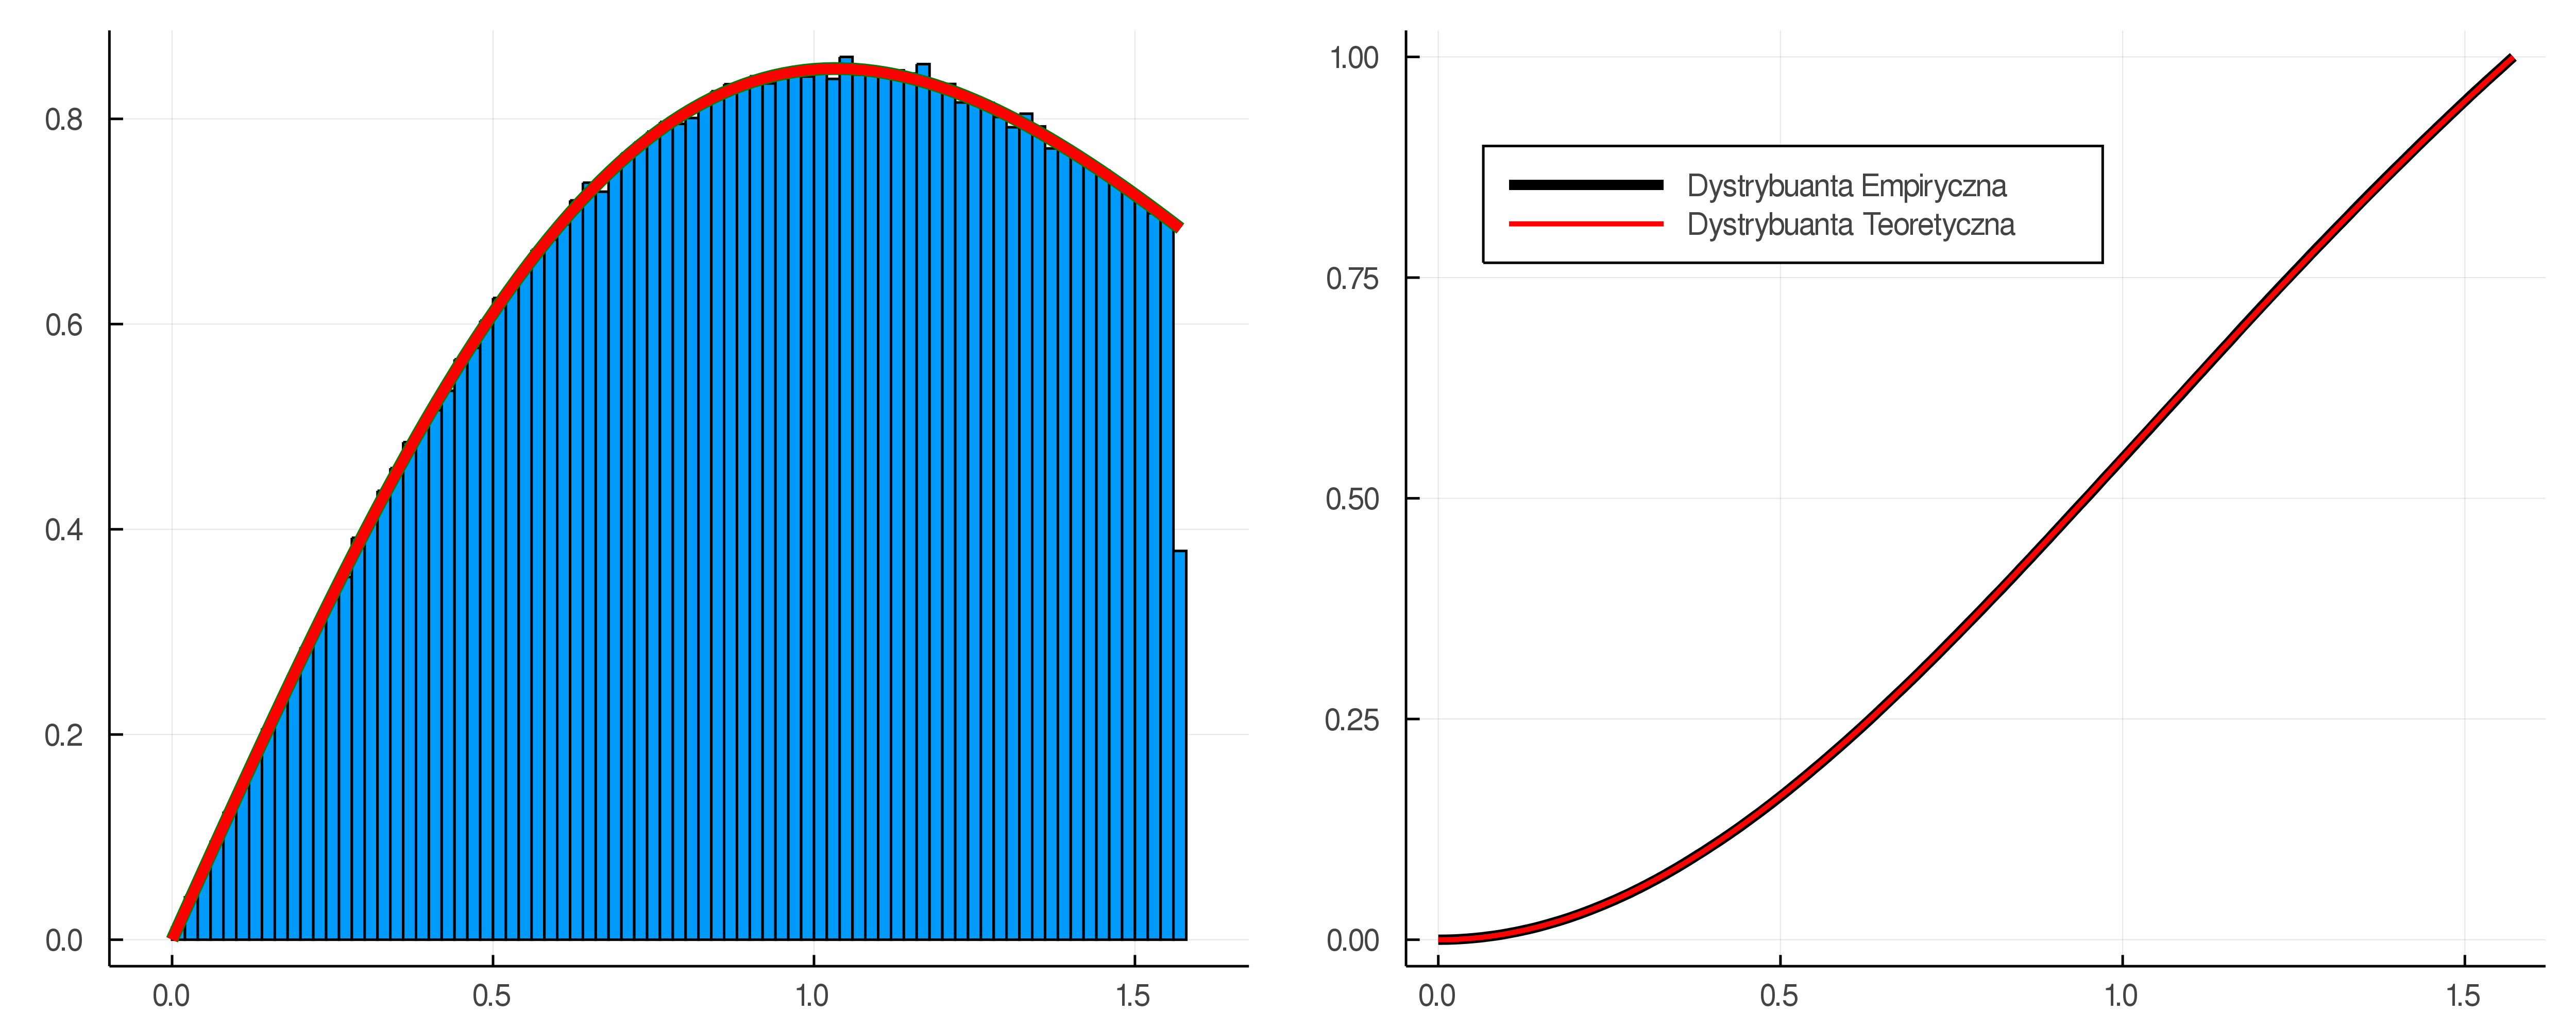
\includegraphics[width=\columnwidth]{fig/fig_AO_con.png}
	\end{figure}










%%%%%%%%%%%%%%%%%%%%%%%%%%%%%%%%%%%%%%%%3
	
	\section{Metoda splotowa - Malec}
	\subsection{Opis}
	\noindent Metoda ta pozwala wygenerować pewną zmienną losową $X$, przy pomocy innych zmiennych, które potrafimy efektywnie generować, i zsumowaniu ich. Załóżmy, że
	$$ X \buildrel{d} \over{=} Y_1 + Y_2 + \dots + Y_n, $$
	gdzie $Y_i$ to zmienne losowe niezależne. Wtedy algorytm wygląda następująco:
	\begin{enumerate}
		\item Generuj $ Y_1, Y_2, \dots, Y_n $.
		\item Zwróć $ X = Y_1 + Y_2 + \dots + Y_n $.
	\end{enumerate}
	\subsection{Przykłady}
	\subsubsection{Dyskretny - }
	\subsubsection{Ciągły - rozkład chi-kwadrat}
	\noindent Niech $ X \sim \mathcal{X}^2(n) $ oraz niech $Y_1, Y_2, \dots, Y_n$ będzie ciągiem niezależnych zmiennych losowych o rozkładzie normalnym standardowym. Wtedy
	$$ X \buildrel{d} \over{=} Y_1 + Y_2 + \dots + Y_n $$
	Stąd otrzymujemy algorytm:
	\begin{enumerate}[leftmargin=10mm]
		\item Generuj $ Y_1, Y_2, \dots, Y_n $, gdzie $Y_i \sim \mathcal{N}(0, 1) $.
		\item Zwróć $ X = Y_1 + Y_2 + \dots + Y_n $.
	\end{enumerate}
	
	\section{Metoda kompozycji - Malec}




%%%%%%%%%%%%%%%%%%%%%%%%%%%%%%%%%%%%%%%%4
	
	\section{Metoda Boxa-Mullera\textsuperscript{\cite{box-kox}} - Budnik}
	\subsection{Opis}
	
	
	
	\subsubsection{Algorytm}
	\begin{enumerate}[leftmargin=10mm]
		\item Generuj zmienne $U_1, U_2$ - iid, $U_1\sim\mathcal{U}(0,1)$
		\item Zwróć:
		\begin{equation}
			\begin{split}
				X=\sqrt{-2\ln(U_1)}\cos\left(2\pi U_2\right)\\
				Y=\sqrt{-2\ln(U_1)}\sin\left(2\pi U_2\right)
			\end{split}
		\end{equation}
	\end{enumerate}
	
	
	
	\section{Metoda biegunowa\textsuperscript{\cite{polar}} - Budink}
	\subsection{Opis}



	\subsubsection{Algorytm}
	\begin{enumerate}[leftmargin=10mm]
		\item Generuj zmienne $V_1, V_2$ - iid, $V_1\sim\mathcal{U}(-1,1)$
		\item Wyznacz $R^2=V_1^2+V_2^2$
		\item Jeżeli $R^2\ge 1$ wróć do 1.
		\item Zwróć
		\begin{equation}
			\begin{split}
				X=\sqrt{\frac{-2\ln R^2}{R^2}}V_1\\
				Y=\sqrt{\frac{-2\ln R^2}{R^2}}V_2
			\end{split}
		\end{equation}
	\end{enumerate}
	
	\subsection{Szybkość algorytmu}
	Liczba powtórzeń tego algorytmu potrzebna do wygenerowania zmiennej losowej wynosi $\frac{4}{\pi}\approx1.25$.



	
	\section{Zakończenie - Początek}
	
	
	\begin{thebibliography}{1}
		\bibitem{AO - dyskretny}
		\url{https://youtu.be/NFmbgbyj5M0?t=1323}
		
		\bibitem{AO - ciagly}
		\url{https://youtu.be/SpPS0CnhvrE?t=37}
		
		\bibitem{splot}
		\url{https://youtu.be/SpPS0CnhvrE?t=4081}
		
		\bibitem{kompozycja}
		\url{https://youtu.be/7lOH982wrwo?t=50}
		
		\bibitem{box-kox}
		\url{https://youtu.be/7lOH982wrwo?t=1896}
		
		\bibitem{polar}
		\url{https://youtu.be/7lOH982wrwo?t=3349}

	\end{thebibliography}
	
\end{document}